
\chapter{Vervaardigingsplan}
\label{Vervaardigingsplan}
\textit{In dit hoofdstuk wordt het vervaardigingsplan ontwikkeld. Hier wordt de tijdsplanning en het tijdsverloop voor de assemblage besproken. De volgende vragen worden beantwoord: Hoe komt men aan het benodigde materiaal en gereedschap? Door wie, waar en wanneer wordt er aan het pakkethondje gewerkt?}

\section{Benodigde materialen}
\label{Benodigde_materialen}
In \cref{fig:maaklijst} en \cref{fig:kooplijst} staan de maak- en kooplijsten. Deze onderdelen moeten uiteraard samen worden geassembleerd. De meeste componenten worden vastgemaakt met een schroefverbinding, deze kunnen met de hand of met een moersleutel worden aangedraaid. Andere verbindingen in het pakkethondje zijn lasvebindingen voor de kapjes van de wielen en klinkverbindingen voor smalle ruimten. \\
\vspace{\baselineskip}
Het gereedschap dat nodig is:
\begin{center}
 \begin{tabular}{| l | c | r |}  
 \hline
\textbf{Gereedschap} & \textbf{Beschikbaarheid} \\
  Moersleutel          & IWS                      \\
  Hamer                & IWS                      \\
  Boormachine          & IWS                      \\
  Freesmachine         & IWS                      \\
  Lasapparaat          & IWS                      \\
  Popnageltang         & IWS                      \\
  Lasersnijder         & IWS                      \\
  3D-printer           & IWS/ Zelf beschikbaar    \\
  Smeerolie            & IWS/ Bouwmarkt       \\
  \hline
 \end{tabular}
\end{center}

%\begin{center}
% \begin{tabular}{| l | c | r | }
%  \hline			
%  score: & concept: & punten:\\
%  1 & Inklapper & 184 \\
%  2 & Vierpoter & 180 \\
%  3 & Mantis Car & 174 \\
%  4 & Uitschuiver & 165 \\
%  \hline  
% \end{tabular}
%\end{center}
%\vspace{\baselineskip}
\section{Lasersnijden}
\label{se:lasersnijden}
Een groot deel van de onderdelen worden met een lasersnijder uit aluminium- en staalplaat gesneden. De U-profielen en hoekprofielen worden vervolgens gebogen tot de gewenste vorm. Dit zorgt ervoor dat er minder onderdelen moeten worden besteld en de kosten lager zijn. Ook heeft dit het voordeel dat alle boorgaten van tevoren zijn gemaakt. De onderdelen die moeten worden gelasersneden zijn in Solidworks gemodelleerd en worden in een DXF-bestand naar de IWS gestuurd.

\section{Lassen}
\label{se:Lassen}
Voor het lassen moeten de zogenaamde U-kapjes waar de wielen aan zijn verbonden worden gelast aan de schaarlift, zie \cref{fig:U-kapjes}. Er zijn twee redenen voor het kiezen van een lasverbinding. Ten eerste zullen hier de grootste krachten plaatsvinden. Ten tweede is het lastig om andere verbindingstechnieken zoals boutverbindingen toe te passen omdat de afmetingen te klein zijn om daar met een moersleutel te komen.

\begin{figure}[H]
    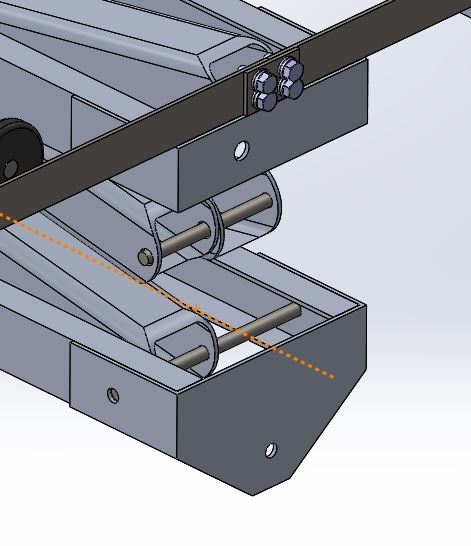
\includegraphics[width = 80mm]{04_vervaardigingsplan/U-kapjes.JPG}
    \caption{U-kapjes, zonder wiel}
    \label{fig:U-kapjes}
\end{figure}

\section{Frezen}
\label{se:Frezen}
Voor het frezen zullen het spindelblokje en de stuurblokjes met een freesmachines worden bewerkt. Dit is omdat deze onderdelen zeer accurate afmetingen hebben die niet kunnen worden besteld. Dit is vooral belangrijk voor de stuurblokjes omdat de precisie van de afmetingen direct invloed hebben op de wendbaarheid van het pakkethondje, zie \cref{fig:stuurblokjes}.


\begin{figure}[H]
    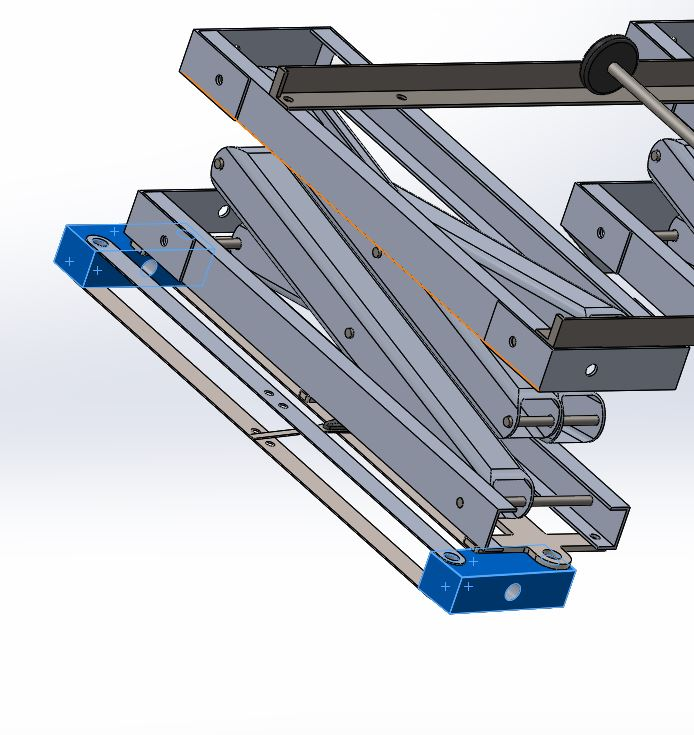
\includegraphics[width = 80mm]{04_vervaardigingsplan/Stuurblokjes.JPG}
    \caption{Stuurblokjes}
    \label{fig:stuurblokjes}
\end{figure}


\section{Overige processen}
\label{se:Overige_processen}
In deze paragraaf worden de overige assemblageprocessen behandeld.
\\
\textbf{Boormachine}\\
De kokerprofielen van de schaarlift bevatten nog geen boorgaten voor de assen, deze zullen dus met een boormachine moeten worden gemaakt in de IWS.
\\
\textbf{3D-printen}\\
De kunststof blokjes aan de bovenkant van de schaarlift zullen worden geprint met een 3D-printer. Deze wordt beschikbaar gesteld door een van de groepsleden.
\\
\textbf{Klinknagels} \\
Voor verbindingen die te smal zijn voor een boutverbinding worden popnagels toegepast. Deze kunnen via één kant worden aangebracht, wat ideaal is voor smalle stukken. Dit is een materiaalgesloten verbinding, wat voordelen en nadelen heeft. Het voordeel van popnagels is dat het gemakkelijk aan te brengen is een zeer sterk is. Het nadeel ervan is dat het niet demontabel is.

\section{Tijdsplanning vervaardiging}
\label{se:planning_vervaardiging}
Er zijn in totaal vijf momenten waar er aan het pakkethondje kan worden gewerkt in de IWS. Hier volgt de planning voor het vervaardigen en assembleren van het pakkethondje:

\begin{table}[H]
\begin{tabular}{| l | l |}
\textbf{IWS moment} & \textbf{Taken}                                                       \\
1                   & Boorgaten maken in kokerprofielen, \newline frezen van belangrijke onderdelen \\
2                   & Schaarliften en platform assembleren                                 \\
3                   & Verder met schaar en platform, lassen, stuursysteem assembleren      \\
4                   & Stuursysteem afronden, geheel in elkaar zetten                       \\
5                   & Geheel in elkaar zetten 
\end{tabular}
\end{table}